\documentclass[12pt]{article}
\usepackage[english]{babel}
\usepackage{graphicx, amsmath, amsfonts, amsthm, mathtools, listings, color, caption, rotating, subfigure, fullpage, textcomp, enumerate, float, listings, MnSymbol, wasysym}

\lstset{
	language=R,
	keywordstyle=\bfseries\ttfamily\color[rgb]{0,0,1},
	identifierstyle=\ttfamily,
	commentstyle=\color[rgb]{0.133,0.545,0.133},
	stringstyle=\ttfamily\color[rgb]{0.627,0.126,0.941},
	showstringspaces=false,
	basicstyle=\tiny,
	numberstyle=\scriptsize,
	numbers=left,
	stepnumber=1,
	numbersep=10pt,
	tabsize=2,
	breaklines=true,
	breakatwhitespace=false,
	aboveskip={1.5\baselineskip},
  columns=fixed,
  upquote=true,
  extendedchars=true,
}

\begin{document}
\begin{center}
STA250, Homework 3 \\
Christopher Aden\\
November 23, 2013\
\end{center}

\section{Basic Optimization:}
\subsection*{Bisection Method}
Coding the bisection algorithm is incredibly simple (algorithm description taken from Rex Cheung's lecture notes):

\begin{enumerate}
\item Find $l$ and $u$ such that $g(l)g(u) < 0$. By the Intermediate Value Theorem, there exists a root between $l$ and $u$. Set iteration counter, $t=0$.
\item If $t$ is equal or greater than max number of iterations, stop and return a null value. Declare non-convergence.
\item Set $c = \frac{l+u}{2}$, compute $g(c)$.
\item If $|g(c)| < \epsilon$ for some small $\epsilon>0$, convergence is reached--return $c$.
\item Otherwise, if $g(l)g(c) < 0$, set $u = c$, else set $l = c$. 
\item $++t$.
\item Goto 2.
\end{enumerate}
The code takes in an arbitrary function $g$, as well as boundary points satisfying the condition outlined in step one of the algorithm. These can be found through guess and check or plugging in the boundaries of the support of the function (not always possible, if the function is supported on the whole real line). It also takes a tolerance $\epsilon$, a maximum number of iterations before stopping and declaring non-convergence, and a debug flag that when enabled, prints values useful in debugging the function.

\subsection*{Newton-Raphson}
%\begin{figure}[H] \center
%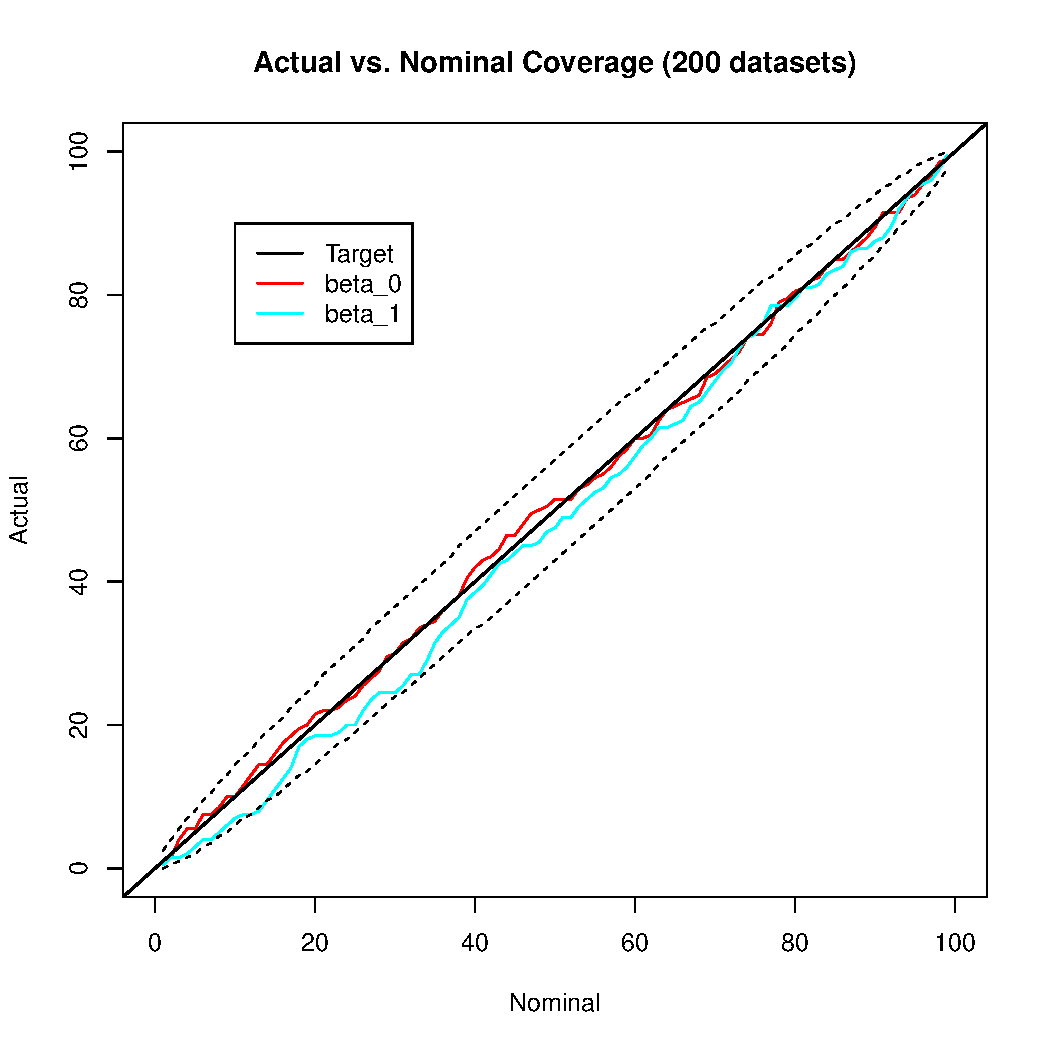
\includegraphics[scale=.65]{coverage_line_plot.pdf}
%\caption*{Coverage Line Plot for $(\beta_1, \beta_2)$, $n=5 \cdot 10^5$, $\text{burn}=10^4$, $\text{retune}=10^3$.}
%\end{figure}
Coding the Newton-Raphson algorithm is a little less simple, but still pretty fast (algorithm description taken from Rex Cheung's lecture notes):

\begin{itemize}
\item Pick $x_0$, set $t = 0$.
\item If $t$ is equal to the max number of iterations, stop and return a null value, declaring non-convergence.
\item Update $x_{t+1} = x_t - \frac{g(x_t)}{g'(x_t)}$.
\item If $|g(x_{t+1})| < \epsilon$, stop. Else, $++t$.
\item Goto 2.
\end{itemize}
The code takes in an arbitrary function $g$, its derivative $g'$, a starting point $x_0$, tolerance $\epsilon$, and the maximum number of iterations and debug flag, identical to the bisection method.

\subsection*{Comparison of Bisection and Newton-Raphson: Linkage Problem}
We compare the results of the two optimization algorithms by testing them on a problem. Define $\lambda = 1 - 2\theta + \theta^2$, where $\theta \in (0,1)$. We want to maximize 
\[ L(\lambda) \propto (2+\lambda)^{125} (1-\lambda)^{18+20} \lambda^{34} \]
From calculus, note that this is equivalent to find the root of the derivative of the log-likelihood.
\[ log(L)' (\lambda) \propto \frac{\partial}{\partial \lambda} \left( 125 log(2+\lambda) + 38 log(1-\lambda) + 34 log(\lambda) \right) \]
\[ \Rightarrow log(L)' (\lambda) \propto \frac{125}{2+\lambda} + \frac{38}{1-\lambda} + \frac{34}{\lambda} \]
We want to find the root of this function (for what value of $\lambda$ this derivative takes the value zero). To do bisection, we just need to find two points, $(l, u)$, such that $log(L)'(l) \cdot log(L)'(u) < 0$.  Two suggested points that worked were $l= .5$ and $u=.8$. Bisection reached convergence (settling on $\lambda = 0.6268215$ after 22 steps).

Newton-Raphson required a second derivative of the log-likelihood. The second derivative is given by
\[ log(L)''(\lambda) \propto \frac{-125}{(2+\lambda)^2} - \frac{38}{(1-\lambda)^2} - \frac{34}{\lambda^2}. \]
Using the starting value of $x_0 = .8$ and tolerance $10^{-5}$, Newton-Raphson also converged (5 iterations, settling on $\lambda = 0.6268215$. 

It should be clear that Newton-Raphson drastically outperformed the Bisection method in terms of number of iterations, but the computation involved in each step was more than bisection, so the comparisons is apples-to-oranges. Using the rbenchmark package in R, We run 10,000 replications of the optimization. The results indicated that bisection took more than twice as long as Newton-Raphson, confirming our belief that Newton-Raphson is a faster algorithm, despite the greater computational cost in each iteration. We may have deduced this from the asymptotic convergence rates, but run time checks aren't a bad idea.
\begin{table}[H] \center \small
\begin{tabular}{rlrrrrrrr} \hline
 & test & replications & elapsed & relative & user.self & sys.self & user.child & sys.child \\ 
  \hline
1 & bisection & 10000 & 3.55 & 2.28 & 3.58 & 0.08 & 0.00 & 0.00 \\ 
2 & Newton-Raphson & 10000 & 1.56 & 1.00 & 1.51 & 0.10 & 0.00 & 0.00 \\ \hline
\end{tabular}
\end{table}

Let's take a look at the likelihood function to see how accurate they were.
\begin{figure}[H] \center
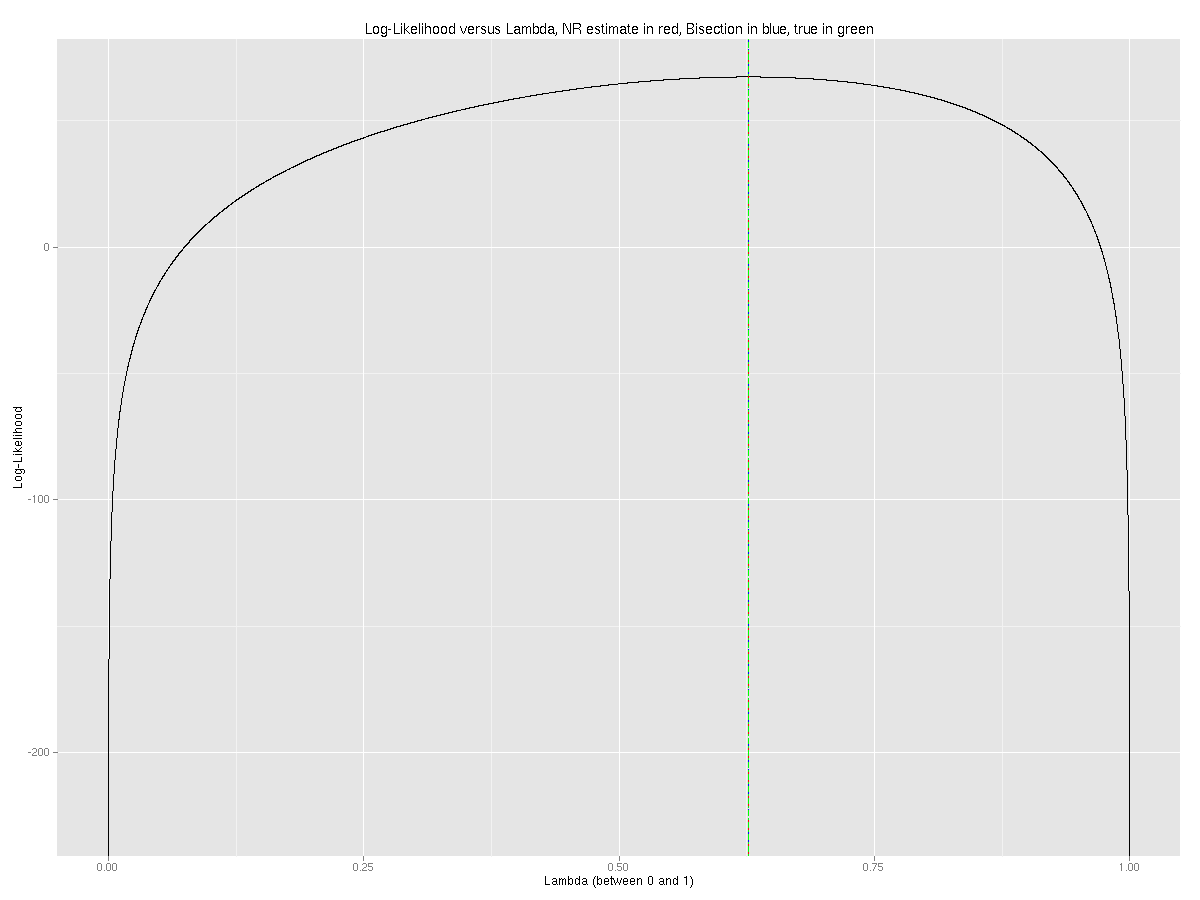
\includegraphics[scale=.40]{Optimizations/LogLike.png}
\caption*{Location of true MLE, Newton-Raphson optimizer and Bisection optimizer, plotted on log-likelihood}
\end{figure}

Both methods managed to hit the true MLE (determined through the woefully inefficient grid search, for completeness) dead on. This demonstrates that finding the root of the derivative is an effective method for finding the extrema of a function iteratively when the extremum cannot be easily determined.

\newpage
\section*{R Source Code}
Code to compute the Newton-Raphson and Bisection Algorithms, along with the code to produce the GGPlot and benchmarking.
\lstinputlisting{"Optimizations/optimizations.R"}
\end{document} 